\documentclass[12pt,a4paper]{article}


\usepackage[brazil]{babel}
\usepackage{enumerate}
\usepackage{amsmath}
\usepackage{amssymb}
\usepackage{xspace}
\usepackage{float}
\usepackage{multirow}
\usepackage{bbding}
\usepackage{lipsum}
\usepackage{graphicx}
\usepackage{pgf,tikz,pgfplots}
\pgfplotsset{compat=1.15}
\usepackage{mathrsfs}
\usetikzlibrary{arrows}
\pagestyle{empty}
\usepackage{setspace}
\usepackage{xcolor}
\usepackage{geometry}
\usepackage[T1]{fontenc}
\usepackage{fancyvrb}


\usetikzlibrary{arrows}

\pagestyle{empty}
\pgfplotsset{compat=1.15}

\newtheorem{lema}{\bf Lema}[section]
\newtheorem{teorema}[lema]{\bf Teorema}
\newtheorem{exemplo}[lema]{\bf Exemplo}
\newtheorem{definição}[lema]{\bf Definição}
\newtheorem{proposição}[lema]{\bf Proposição}
\newtheorem{observação}[lema]{\bf Observação}
\newtheorem{corolário}[lema]{\bf Corolário}
\newenvironment{demonstração}{\noindent {\bf Demonstra\c{c}\~{a}o:}}{\hfill${\blacksquare}\hspace*{-2.8mm}{\sqcup} $ \newline}
\newcommand{\Dem}{{\bf Demonstração}\quad}
\newcommand{\cqd}{{\hfill $\rule{2.0mm}{2.0mm}$}\vspace{0.1cm}}


\geometry{a4paper, left=2cm, right=2cm, top=2cm, bottom=2cm}

\begin{document}
	
\begin{figure}[htb]
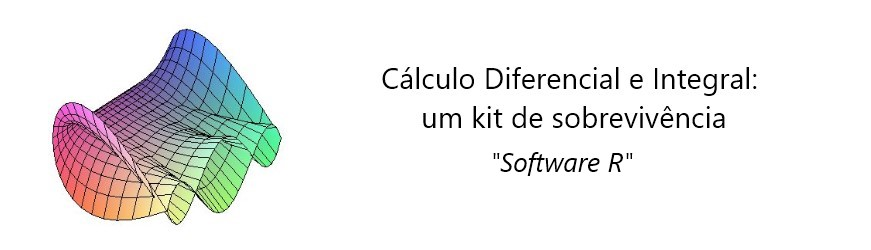
\includegraphics[scale=0.6]{logo.jpg}
\end{figure}

	
	
	\begin{center}Lucas Stefano Xavier de Sousa \\ Orientador: Prof. Dr. Rodrigo Martins.\end{center}
	
	
	\vspace{2cm}
	
	\section*{Desvio Padrão}
	
	O desvio padrão é uma medida de dispersão (medidas de dispersão, são medidas  que indicam o grau de dispersão, ou variabilidade do conjunto de  observações pesquisados, em relação a uma medida de posição) que indica o quanto o conjunto de dados é uniforme, ele é definido como a raiz quadrada da variância e é representado por:\\
	
	\begin{center}									
		\vspace{0.2cm}
		\begin{tabular}{|c||c|}
			\hline
			\textit{\textbf{Amostral:}} & \textbf{Populacional:} \\
			$s= \sqrt{s^2}$             &  $	\sigma= \sqrt{\sigma^2}$; \\
			\hline
		\end{tabular}
	\end{center}

	
	
	\section*{Utlizando Desvio Padrão no R:}
	
	Para calcular o desvio padrão no R, podemos utilizar a função \textbf{sd}. Essa função faz parte do pacote \textbf{stats} e já está instalado de forma nativa no R.\\
	Uma outra forma de se calcular o desvio padrão é aplicando a função da raiz quadrada. \\


	\subsection*{Exemplo 1: Função sd para o conjunto de dados \c(1, 2.5, 7, 5, 10)}

	\begin{verbatim}
		> library(stats)
		> x <- c(1, 2.5, 7, 5, 10) #Conjunto de dados aleatórios
		# Calculando o desvio padrão através da função sd do pacote Stats
		> sd(x)
		[1]  3.577709 # Resultado do desvio padrão
	\end{verbatim}
	
	\subsection*{Exemplo 2: Raiz da Variância, utlizando a função nativa variância}
	
	\begin{verbatim}
		> x <- c(1, 2.5, 7, 5, 10) #Conjunto de dados aleatórios
		# Calculando através da raiz de variância
		> sqrt(var(x))
		[1]  3.577709 # Resultado do desvio padrão
		\end{verbatim}

	
	\bibliographystyle{apalike}
	\begin{thebibliography}{100}
		
		\bibitem {Magalhães} Magalhães, Marcos Nascimento and Lima, Antonio Carlos Pedroso de. Noções de probabilidade e estatística. EDUSP: Ed. 2015.
		\bibitem{R Core Team} R Core Team. R: A Language and Environment for Statistical Computing, 2021.
	\end{thebibliography}
	
\end{document}